\documentclass[12pt]{article}
\usepackage{tikz, setspace, indentfirst}
\usepackage[margin=1in]{geometry}

\usetikzlibrary{decorations.pathreplacing, calc}

\definecolor{lightBlue}{RGB}{173,221,237}

\begin{document}

\setstretch{1.3}

The World Health Organization (WHO) recently urged countries to impose taxes on sugary drinks in order to combat obesity, diabetes, and tooth decay. Their contention is that a tax increasing their prices by 20\% would reduce proportionately their consumption. 

\vspace{\baselineskip}

Define an externality as a side effect of consumption or production not taken into account by the consumer or producer, that affects the costs and utility of other consumers and producers. A demerit good is one that is socially undesirable and exhibits negative consumption or production externalities. Sugary drinks are therefore demerit goods since they exhibit negative externalities in consumption. Their consumption is associated with the aforementioned negative health effects on consumers|effects that consumers do not necessarily consider as they consume the drinks. Society also considers other effects: the increased demand on its healthcare system, the lost productivity that arises from potential decay in the quality of labour, and other external costs of consumption. In fact, social benefit is equal to private benefit minus the external costs of the consumption, so social benefit $<$ private benefit.

\vspace{\baselineskip}

\begin{center}

\ \ \ \ \ Figure 1. Market for sugary drinks

	\vspace{0.5\baselineskip}

	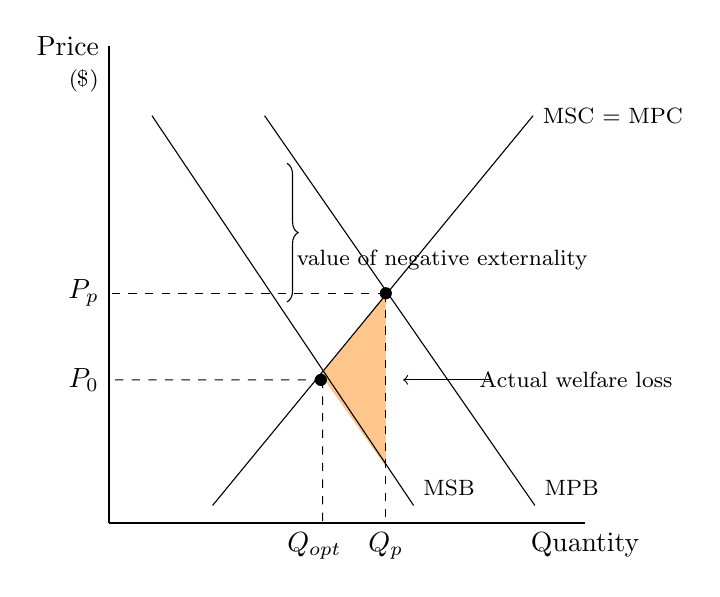
\begin{tikzpicture} [scale = 1.1]
	
		% Define coordinates.

	%axes

	\coordinate (origin) at (0,0);
	\coordinate [label= left:$\textrm{Price}$] (P) at (0, 5.5);
	\coordinate [label= below:$\textrm{Quantity}$] (Q) at (5.5, 0);
	
	%demand curve
	\coordinate (demandTail) at (0.5, 4.7);
	\coordinate [label= above right:\footnotesize $\textrm{MSB}$, xshift = -15pt] (MSB) at (4.0, 0.2);
	
	\coordinate (demandTail1) at (1.8, 4.7);
	\coordinate [label= above right:\footnotesize $\textrm{MPB}$, xshift = -15pt] (MPB) at (5.4, 0.2);
	
	%supply curve 1
	\coordinate (supplyTail1) at (0.2, 0.2);
	%[label= right:$S_1$]
	\coordinate (S) at (4, 4.7);
	
	%supply curve 0 
	\coordinate (supplyTail0) at (1.2, 0.2);
	\coordinate [label = right:\footnotesize $\textrm{MSC = MPC}$] (S0) at (4.9, 4.7);
	
	%Equilibria 
	\coordinate (E1) at (2.05, 2.4);	
	\coordinate (E2) at (2.47, 1.65);
	
% Colour in.

	\fill [fill=orange!45] (3.2, 2.65) -- (3.2, 0.65) -- (2.45, 1.71) -- cycle;
	 
% Draw axes.

	\draw[thick] (origin) -- (P);
	\draw[thick] (origin) -- (Q);  
	
% Draw lines.
		
	\draw (demandTail) -- (MSB);
	\draw (demandTail1) -- (MPB);
	%\draw (supplyTail1) -- (S);
	\draw (supplyTail0) -- (S0);
	
	\draw[dashed] (3.2, 2.65) -- (3.2, 0) node[below] {$Q_p$};
	
	\draw[dashed] (E2) -- (2.47, 0) node[below, xshift=-3pt] {$Q_{opt}$};
	\draw[dashed] (E2) -- (0, 1.65) node[left] {$P_0$};
	
	\draw[dashed] (3.2, 2.65) -- (0, 2.65) node[left] {$P_p$};
	
	
	%\draw[thick, ->]($(S0) + (-0.5, -0.5)$) -- ($(S) + (-0.3, -0.5)$);
	
% Draw points of equilibria. 

	\fill[black] (3.2, 2.65) circle (2pt);
	\fill[black] (2.45, 1.65) circle (2pt);

	
% Draw label arrows.

	%\draw[thick, ->] (-0.8, 1.65) -- (-0.8,2.4);
	\draw[->] (4.4, 1.65) -- (3.4, 1.65) node [right, xshift = 24pt] {\footnotesize Actual welfare loss} ;
	
	
	\draw [decorate, decoration ={brace,amplitude=4pt},xshift=-4pt,yshift=0pt] (2.2, 4.15) -- (2.2, 2.55) node [right, yshift = 15pt] {\footnotesize value of negative externality};
	
	\draw (0, 5.1) node [left]{\footnotesize (\$)};
	
	\end{tikzpicture}
	
\end{center}

In Figure 1, this relationship is represented as the vertical difference between the marginal private benefit (MPB) curve and the marginal social benefit (MSB) curve, which are analogous to demand from different perspectives. At all quantities, for every incremental unit of sugary drinks consumed, the utility derived by private consumers exceeds that derived by society. Next, the intersection between the marginal benefit curves and the marginal cost curves, social (MSC) and private (MPC), are at different quantities (these curves coincide in the figure): $Q_p$ in the free market and $Q_{opt}$ if it were up to society to decide production and consumption. Finally, the shaded triangle represents an actual welfare loss being the result of overproduction on sugary drinks. In the free market, sugary drinks are still produced and consumed even at the point where MSC $>$ MSB. Therefore, the market has failed to allocate resources in a way that maximizes social welfare.


\vspace{\baselineskip}

With a tax levied on sugary drinks, marginal private costs will increase. This is illustrated in Figure 2 as an upward shift of the MPC curve from $\textrm{MPC}_0$ to $\textrm{MPC}_1$, so that at every quantity, the free market perceives the incremental cost of production to be higher.

\vspace{\baselineskip}

\begin{center}

\ \ \ \ \ Figure 2. Market for sugary drinks

	\vspace{0.5\baselineskip}

	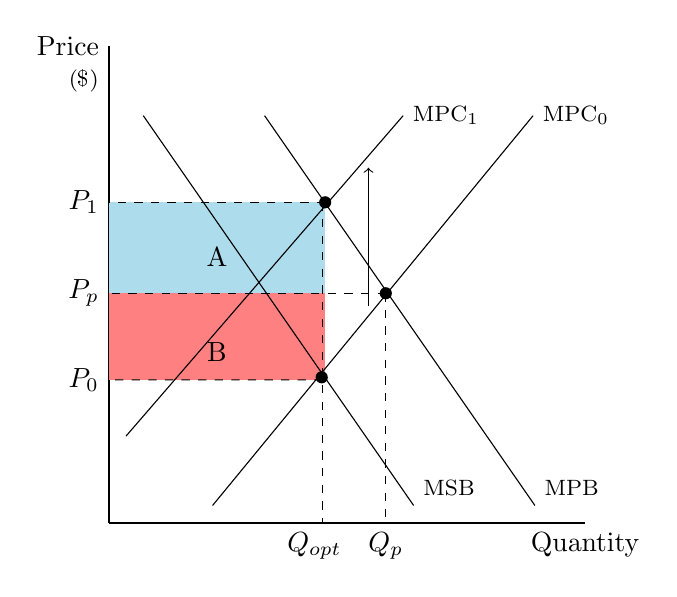
\begin{tikzpicture} [scale = 1.1]
	
		% Define coordinates.

	%axes

	\coordinate (origin) at (0,0);
	\coordinate [label= left:$\textrm{Price}$] (P) at (0, 5.5);
	\coordinate [label= below:$\textrm{Quantity}$] (Q) at (5.5, 0);
	
	%demand curve
	\coordinate (demandTail) at (0.4, 4.7);
	\coordinate [label= above right:\footnotesize $\textrm{MSB}$, xshift = -15pt] (MSB) at (4.0, 0.2);
	
	\coordinate (demandTail1) at (1.8, 4.7);
	\coordinate [label= above right:\footnotesize $\textrm{MPB}$, xshift = -15pt] (MPB) at (5.4, 0.2);
	
	%supply curve 1
	\coordinate (supplyTail1) at (0.2, 1);
	\coordinate [label= right:\footnotesize $\textrm{MPC}_1$] (S1) at (3.4, 4.7);
	
	%supply curve 0 
	\coordinate (supplyTail0) at (1.2, 0.2);
	\coordinate [label = right:\footnotesize $\textrm{MPC}_0$] (S0) at (4.9, 4.7);
	
	%Equilibria 
	\coordinate (E1) at (2.05, 2.4);	
	\coordinate (E2) at (2.47, 1.65);
	 
% Draw axes.

	\draw[thick] (origin) -- (P);
	\draw[thick] (origin) -- (Q); 
	
% colour

	\fill [fill=lightBlue] (0, 3.7) rectangle (2.5, 2.65); 
	\fill [fill=red!50] (0, 2.65) rectangle (2.5, 1.65);
	
% Draw lines.
		
	\draw (demandTail) -- (MSB);
	\draw (demandTail1) -- (MPB);
	\draw (supplyTail1) -- (S1);
	\draw (supplyTail0) -- (S0);
	
	\draw[dashed] (3.2, 2.65) -- (3.2, 0) node[below] {$Q_p$};
	
	\draw[dashed] (2.5, 3.7) -- (0, 3.7) node[left] {$P_1$};
	
	\draw[dashed] (2.47, 3.7) -- (2.47, 0) node[below, xshift=-3pt] {$Q_{opt}$};
	\draw[dashed] (E2) -- (0, 1.65) node[left] {$P_0$};
	
	\draw[dashed] (3.2, 2.65) -- (0, 2.65) node[left] {$P_p$};
	
	\draw[->] (3, 2.5) -- (3, 4.1);
	
	
	%\draw[thick, ->]($(S0) + (-0.5, -0.5)$) -- ($(S) + (-0.3, -0.5)$);
	
% Draw points of equilibria. 

	\fill[black] (3.2, 2.65) circle (2pt);
	\fill[black] (2.46, 1.68) circle (2pt);
	\fill[black] (2.5, 3.7) circle (2pt);
	
	\draw (1.25, 2.85) node[above] {A};
	\draw (1.25, 1.75) node[above] {B};
	
	\draw (0, 5.1) node [left]{\footnotesize (\$)};

	
% Draw label arrows.

	%\draw[thick, ->] (-0.8, 1.65) -- (-0.8,2.4);
	
	\end{tikzpicture}
	
\end{center}

The taxation aims to increase MPC, allocating resources away from the market to maximize social welfare and decrease production. Hence, should the new quantity traded be $Q_{opt}$, (intersection of $\textrm{MPC}_1$ and MPB), social welfare will be maximized.

\vspace{\baselineskip}

While the taxation may theoretically remove the welfare loss in the market, the policy\rq s practicality is questionable. It is  uncertain that decreasing the consumption of sugary drinks will reduce the negative health effects of consumption that burden society. This is because there are many reasons that people become obese, or get diabetes or tooth decay|reasons other than overconsumption of sugary drinks. Moreover, the food industry naturally resists such taxation. For instance, the article mentions a soda tax in New York City that was struck down in court.


\vspace{\baselineskip}

Normally, the value of a negative externality is impossible to quantify. This is significant because the taxation policy can only fully quell the welfare loss if the market is taxed by the value of the externality. If it is taxed too heavily and MPC moves too far to the left, there exists a potential welfare gain. Furthermore, parallel markets may emerge, requiring government expenditure to police them. If it is taxed at too low a rate, an actual welfare loss still exists. Despite this, a panel of experts, after extensively reviewing scientific literature and producing mathematical models, claim to have quantified the effects of such a tax. Essentially, they can predict the resulting reduced production with the taxation. Nonetheless, it remains unknown as to what $Q_{opt}$ is, and thus, the ideal amount to tax is still unquantified.

\vspace{\baselineskip}

Overall, consumers will find that the taxation makes every unit of sugary drink more expensive. Here, consumers will have to pay an additional $P_1 - P_p$ dollars on every unit. This gives them a tax burden that can be represented by area $A$ in Figure 2: $(P_1 - P_p) \times Q_{opt}$. Concurrently, producers lose potential revenue, since the amount that they receive for each unit produced decreases with the taxation. Their tax burden can be represented by area $B$: $(P_p - P_0) \times Q_{opt}$. Notice that their new revenue, $P_0Q_{opt}$ is contained within the old, $Q_pP_p$. Finally, governments will find that, as with most addictive goods, taxing sugary drinks is lucrative. Government revenue can be quantified as $(P_1 - P_0) \times Q_{opt}$, or area $A + B$. 

\end{document}
